\chapter{Modelos de Redes Neurais}
\label{ch:03}


% \epigraph{\itshape Those who cannot remember the past are condemned to compute it.''}{---Steven Pinker, \textit{Words and Rules}}

Este capítulo serve como uma introdução à teoria das redes neurais. Os conceitos aqui introduzidos servirão como embasamento teórico imprescindível para a apresentação do modelo final utilizado nesta pesquisa, o \textit{Encoder-Decoder}. 

\section{Introdução a Redes Neurais}

Um modelo de rede neural é, essencialmente, um modelo de aprendizado de máquina supervisionado %[ref] 
que está a procura de identificar padrões. Um modelo de aprendizado de máquina é uma tarefa computacional que explora algoritmos que podem aprender a partir de seus erros e fazer previsões sobre dados. Esse tipo de algoritmo é normalmente inicializado com nenhuma expectativa sobre a tarefa que deve realizar e busca informações exclusivamente a partir dos dados do problema. Os possíveis tipos de aprendizado de máquina são divididos entre: \textit{supervisionados}, \textit{não-supervisionados}
e por \textit{reforço}. (ref)
No caso das redes neurais, o aprendizado diz-se supervisionado, pois informa-se ao modelo o \textit{target} esperado  pelo treinamento (o \textit{alvo}) para cada informação de entrada (cada \textit{input}).

A inspiração para o desenvolvimento da modelagem em redes neurais artificiais surgiu a partir de estudos em neurosciência %[ref] 
que concluíram que, diante de múltiplas apresentações de um mesmo estímulo, um mesmo conjunto de neurônios sofre incitação e dispara. Um estímulo diferente resulta no disparo de um conjunto de neurônios diferente (\cite{hubel:1962}).  Analogamente, o modelo artificial é composto por uma camada denominada de \textit{input} responsável por receber diferentes estímulos (matematicamente retratados por vetores numéricos que representam o objeto do aprendizado). A informação recebida é distribuída ao longo de múltiplas conexões com a próxima camada através de uma multiplicação com uma matriz de pesos $\vect{W}$. A matriz de pesos funciona como uma analogia às conexões existentes entre neurônios de modo que um peso maior representa uma conexão reforçada e um peso menor representa uma conexão reprimida. Além disso, é importante que o sistema de aprendizado não seja demasiado sensível a todo \textit{input} que receber, pois nesse caso cada \textit{input} diferente recebido alteraria completamente o modelo impossibilitando um aprendizado generalizado. Como solução, o resultado obtido a partir da multiplicação dos pesos pelos \textit{inputs} entra como argumento em uma função, que nesse contexto é chamada de \textit{função de ativação}. A função de ativação é uma função que simula o potencial energético existente entre as conexões neurais e permite que uma unidade apenas seja ativada caso o resultado dessa função atinja um limiar mínimo. Isso permite ao sistema a produção de diferentes respostas para padrões diferentes utilizando a mesma rede e além disso, permite que o aprendizado ocorra de forma gradual, de modo que o efeito de estímulos passados ainda perdure por um longo período mesmo após a apresentação de novos estímulos. Uma das funções de ativação mais utilizadas na literatura (e inclusive utilizada pelos pesquisadores Rumelhart e McClelland) é a função \textit{Sigmoid}, uma função suave, diferenciável e facilmente interpretável. A Fig. \ref{fig:sigmoidplot} ilustra o processo de ativação dado um \textit{input} $\vect{x}$. Supõe-se que um neurônio seja ativado apenas se houver uma energia mínima para tal. Da mesma forma, representa-se uma ativação no eixo \textit{y} (com valores entre 0 (não ativação) e 1 (ativação)) de modo que apenas valores mais altos de $\vect{x}$ atingem valores próximos da ativação em \textit{y}.

\begin{figure}[H]
\centering
\scalebox{0.9}{
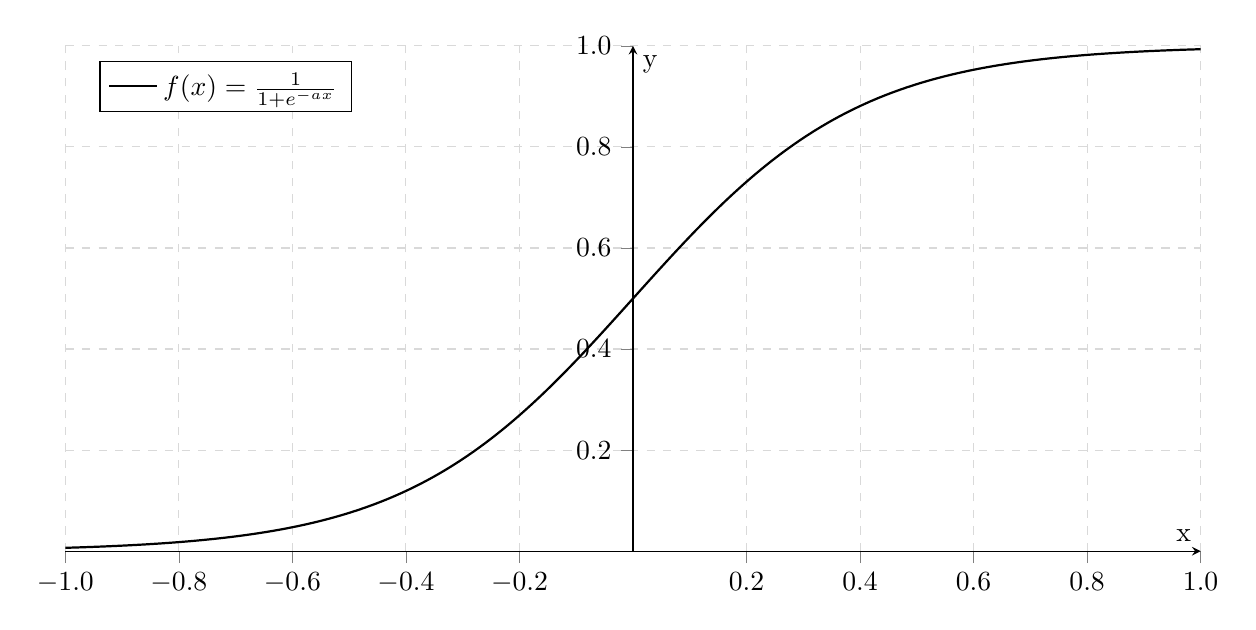
\begin{tikzpicture}
    \begin{axis}[
    	legend pos=north west,
        axis x line=middle,
        axis y line=middle,
        x tick label style={/pgf/number format/fixed,
                            /pgf/number format/fixed zerofill,
                            /pgf/number format/precision=1},
        y tick label style={/pgf/number format/fixed,
                            /pgf/number format/fixed zerofill,
                            /pgf/number format/precision=1},
        grid = major,
        width=16cm,
        height=8cm,
        grid style={dashed, gray!30},
        xmin=-1,     % start the diagram at this x-coordinate
        xmax= 1,    % end   the diagram at this x-coordinate
        ymin= 0,     % start the diagram at this y-coordinate
        ymax= 1,   % end   the diagram at this y-coordinate
        %axis background/.style={fill=white},
        xlabel=x,
        ylabel=y,
        tick align=outside,
        enlargelimits=false]
      % plot the stirling-formulae
      \addplot[domain=-1:1, black, thick,samples=500] {1/(1+exp(-5*x))};
      %\addplot[domain=-1:1, blue, ultra thick,samples=500] {1/(1+exp(-10*x))};
      \addlegendentry{$f(x)=\frac{1}{1+e^{-ax}}$}
      %\addlegendentry{$g(x)=\frac{1}{1+e^{-10x}}$}
    \end{axis} 
\end{tikzpicture}
}
\caption{A função \textit{Sigmoid}.}
\label{fig:sigmoidplot}
\end{figure} %diminuir esse desenho

Após essa passagem pela função de ativação, o resultado serve como novo input para a próxima camada e assim sucessivamente até a última, a camada de \textit{output}. Todas as camadas existentes entre as camadas de \textit{input} e de \textit{output} são chamadas de \textit{camadas escondidas} (Ver Fig. \ref{fig:ffd}.)

% \begin{align}\label{eq:sigmoid}
% p(w_{i} = 1) = \frac{1}{1+e^{\sum_{i} w_{i}x_{i}}}
% \end{align}

Algebricamente, pode-se representar o processo descrito através da composição de múltiplas funções, uma vez que o resultado das operações precedentes servirão como entrada para as próximas camadas.

\begin{align}
% f(\vect{x}) &= f^{(2)}(f^{(1)}(\vect{x}; \vect{W}_1); \vect{W}_2)\\
% &= 
\sigma(\vect{W}_2 (\sigma(\vect{W}_1\vect{x})))
\end{align}

\input{definitions/colors}
\input{definitions/styles}
\begin{figure}[ht!]
\centering

\scalebox{1.0}{
\begin{tikzpicture}[auto]

% operations =========

% FNN input
\node[normal] (x1) {};
\node[textonly, above=10pt of x1] (input) {Camada de \textit{inputs}};
\node[normal, below=10pt of x1] (x2) {};
\node[normal, below=10pt of x2] (x3) {};
\node[normal, below=10pt of x3] (x4) {};
\node[normal, below=10pt of x4] (x5) {};
\node[normal, below=10pt of x5] (x6) {};

% FNN output
\node[textonly, right=50pt of x1] (center) {Camada Escondida};
\node[normal, below=25pt of center] (y1) {};
\node[normal, below=10pt of y1] (y2) {};
\node[normal, below=10pt of y2] (y3) {};

% FNN output
\node[textonly, right=110pt of input] (output) {Camada de \textit{outputs}};
\node[normal, below=15pt of output] (z1) {};

\node[normal, below=10pt of z1] (z2) {};
\node[normal, below=10pt of z2] (z3) {};
\node[normal, below=10pt of z3] (z4) {};
\node[normal, below=10pt of z4] (z5) {};
\node[normal, below=10pt of z5] (z6) {};

% phon features 2

% edges FNN
\path[nedge] (x1) -- (y1);
\path[nedge] (x1) -- (y2);
\path[nedge] (x1) -- (y3);

\path[nedge] (x2) -- (y1);
\path[nedge] (x2) -- (y2);
\path[nedge] (x2) -- (y3);

\path[nedge] (x3) -- (y1);
\path[nedge] (x3) -- (y2);
\path[nedge] (x3) -- (y3);

\path[nedge] (x4) -- (y1);
\path[nedge] (x4) -- (y2);
\path[nedge] (x4) -- (y3);

\path[nedge] (x5) -- (y1);
\path[nedge] (x5) -- (y2);
\path[nedge] (x5) -- (y3);

\path[nedge] (x6) -- (y1);
\path[nedge] (x6) -- (y2);
\path[nedge] (x6) -- (y3);

% edges FNN
\path[nedge] (y1) -- (z1);
\path[nedge] (y1) -- (z2);
\path[nedge] (y1) -- (z3);
\path[nedge] (y1) -- (z4);
\path[nedge] (y1) -- (z5);
\path[nedge] (y1) -- (z6);
\path[nedge] (y2) -- (z1);
\path[nedge] (y2) -- (z2);
\path[nedge] (y2) -- (z3);
\path[nedge] (y2) -- (z4);
\path[nedge] (y2) -- (z5);
\path[nedge] (y2) -- (z6);
\path[nedge] (y3) -- (z1);
\path[nedge] (y3) -- (z2);
\path[nedge] (y3) -- (z3);
\path[nedge] (y3) -- (z4);
\path[nedge] (y3) -- (z5);
\path[nedge] (y3) -- (z6);

\end{tikzpicture}
}\caption{Esquema de uma Rede Neural com Camada Escondida} 
\label{fig:ffd}
\end{figure}

\section{Treinamento}

Para que a rede seja capaz de identificar os padrões desejados, é necessário alimentá-la também com o que se espera como resposta (\textit{targets} ou \textit{alvos}), pois o treinamento da mesma consiste, essencialmente, na atualização das matrizes de pesos que deve ocorrer a partir da comparação entre os valores previstos pela rede (os \textit{outputs}) e os \textit{targets}. A comparação entre esses valores se dá por meio de uma função de custo (\textit{Loss Function}), que representa uma forma de se quantificar o quão perto se está de uma rede ideal em que os resultados previstos correspondam exatamente aos \textit{targets}. O objetivo do aprendizado da rede é minimizar essa diferença, ou seja, encontrar os valores dos pesos na matriz $\vect{W}$ que minimizam a função de custo (\cite{josh:2017}). Para isso, faz-se uso de um algoritmo chamado de \textit{backpropagation} (ref). Após a inserção de cada input e a aplicação do algoritmo de backpropagation, todos os pesos de $\vect{W}$ são atualizados simultaneamente com os valores que em conjunto minimizam a função de custo e portanto aproximam as previsões da rede aos alvos. Entretanto, o ajuste de um modelo de redes neurais é bastante delicado e experimental. Ele depende não somente da busca pelos melhores parâmetros de $\vect{W}$ como também de uma busca pelos chamados \textit{hiperparâmetros}. 

Os hiperparâmetros são parâmetros do modelo que são escolhidos a priori para configurar o modelo. Um deles refere-se ao número de vezes em que um mesmo input é inserido, conhecido como o número de \textit{épocas}. Existem também outros hiperparâmetros importantes como a taxa de aprendizado $\eta$, o parâmetro de regularização $\lambda$, dimensões de camadas escondidas, número de camadas escondidas, entre outros (\cite{josh:2017}). Todos esses hiperparâmetros definem as configurações do treinamento e juntos podem levar ao sucesso ou insucesso do aprendizado. A escolha dos melhores hiperparâmetros para um modelo de redes neurais não é tarefa trivial. Múltiplos treinamentos com diferentes configurações de hiperparâmetros são realizados para que se possa fazer essa escolha. Na prática, porém, é mais comum que esses hiperparâmetros sejam configurados a partir de resultados de experimentos semelhantes publicados na literatura.   

Mesmo com uma extensa busca pelos hiperparâmetros do modelo, nem sempre é possível encontrar valores em $\vect{W}$ que possibilitem o aprendizado de forma satisfatória. Na prática, é bastante comum a ocorrência de problemas conhecidos como \textit{overfit} (quando o modelo se torna especialista nos dados de treino mas tem dificuldade de generalizar para dados nunca vistos antes) e \textit{underfit} (quando o modelo falha em capturar o padrão subjacente dos dados) (\cite{josh:2017}). Na literatura existem algumas técnicas disponíveis para tratar dessas questões, como Dropout, Data Augmentation e Over ou Under Sampling (ref). Ainda assim, o modelo de redes neurais é um modelo cuja interpretabilidade mostra-se ainda bastante inacessível, o que torna o resultado do treinamento bastante hermético. (ref)   %ref 

\section{Uma Outra Arquitetura}
\label{sec:arqFDD}
%juntar o cap 4 aqui dentro
O esquema apresentado pelos pesquisadores Rumelhart e McClelland represetado na Fig. \ref{fig:esquemafdd} é conhecido como uma arquitetura do tipo \textit{Feedforward-Network (FFD)} sem camadas escondidas. Nesse caso, todos os nódulos da camada de input se conectam diretamente aos nódulos da camada de output.

% Com o modelo de RM foi possível atingir uma acurácia de 91\% na tarefa de aprendizado de verbos do Simple Past da língua inglesa. Entretanto a arquitetura do tipo FFD não é a mais adequada para dados sequenciais. No Cap. \ref{ch:02} foi abordado o complicado esquema de codificação dos verbos através de trigramas de traços distintivos. O processo de decodificação dos mesmos era ainda mais complicado e envolvia um esquema de competição entre trigramas (\cite{rumelhart:1986}). \cite{Pinker:1999} inclusive comenta sobre a dificuldade de decodificação da palavra 'algalgal' (uma palavra da língua Oykangand). Como a representação do output da rede FFD aponta apenas a presença ou ausência dos traços, e não quantas vezes eles aparecem, o processo de decodificação apresenta problemas e a rede dificilmente acerta em casos de verbos maiores ou com repetições de trigramas de traços. No caso da língua portuguesa, essa tarefa é bastante difícil pois os verbos são em média maiores que os verbos da língua inglesa (como comentado no Capítulo \ref{ch:01}). 

Com isso, introduz-se um novo tipo de rede conhecida como Rede Neural Recorrente (RNN) cuja arquitetura foi pensada para esse caso de dados sequenciais. Para entender o funcionamento desse tipo de rede, antes faz-se necessária uma introdução ao conceito de \textit{Modelo de Linguagem}.

\subsection{Modelo de Linguagem}

Um modelo de linguagem é um modelo que propõe uma distribuição probabilística para uma sequência de termos em uma linguagem natural (\cite{manning99foundations}).
Em outras palavras, um modelo de linguagem responde à pergunta: “dados os termos $x_1,x_2,x_3,x_4$, qual a probabilidade deles ocorrerem em uma determinada sequência?”

A forma clássica de se abordar esse problema se dá através da assunção de independência entre os termos da sequência em combinação à Regra do Produto de Probabilidades, ou seja, considera-se que a probabilidade de uma determinada sequência com $T$ termos acontecer é igual à probabilidade da $palavra_{t}$ ocorrer dado que as outras $t-1$ palavras ocorreram:

\begin{equation}
P(x_1, \dots, x_T) = \prod_{t=1}^{T} P(x_t \vert x_1, \dots, x_{t-1}) 
\end{equation}

Essas considerações deram origem aos modelos de $N$-Gramas. Diferentes valores para N dão origem a diferentes modelos. O modelo de unigrama, por exemplo, leva em consideração apenas a probabilidade de cada termo da sequência:

\begin{equation}
P_{uni}(x_1, x_2, x_3, x_4) = P(x_1)P(x_2)P(x_3)P(x_4)
\end{equation}

Em que $P(x_i) = contagem(x_i)$ e $contagem$ é uma função que conta a ocorrência dessa palavra no corpus.\\

A partir de N=2, ou seja, do modelo de \textit{bigramas}, esse tipo de modelagem começa a fazer mais sentido. A ideia é calcular a probabilidade dos termos dada a contagem de vezes em que eles ocorreram um após o outro em um corpus de treinamento.

\begin{equation}
P_{bi}(x_1,x_2,x_3,x_4) = P(x_1)P(x_2\vert x_1)P(x_3\vert x_2)P(x_4\vert x_3)
\end{equation} 
em que
\begin{equation}
P(x_i\vert x_j) = \frac{contagem(x_i, x_j)}{contagem(x_j)}
\end{equation}


Esse tipo de modelo de linguagem, apesar de intuitivo, apresenta alguns obstáculos. O primeiro deles é o fato de atribuir probabilidade 0 se uma sequência de termos específica não existe no corpus de treinamento. Outro grande problema é o número alto de computações das probabilidades conforme o texto aumenta de tamanho ou o \textit{N} do \textit{N-Grama} aumenta. Desse modo fica difícil de se manter uma coerência dentro de uma sentença, o que se vê na prática são frases constituídas de “remendos”, pequenos grupos de (\textit{N}) palavras que produzem uma janela muito pequena de sentido.

\subsection{Redes Neurais Recorrentes}
\label{sec:RNN}

Os modelos de Redes Neurais Recorrentes (ref) surgem como uma alternativa ao tradicional modelo de linguagem de \textit{N-Gramas}. A ideia central desse modelo consiste na retroalimentação dos elementos sequenciais, de modo que o \textit{input} de cada um deles serve, não somente para a previsão do próximo item da sequência, mas também para a formação de um componente intermediário, um \textit{estado}. Esses estados, representados na Figura \ref{fig:unfoldedrnn} como $\vect{h}$'s são matrizes que funcionam como uma espécie de memória condensada dos elementos precedentes e servem como input para os estados posteriores. Essa é uma maneira de retransmitir a cada momento os efeitos dos \textit{inputs} anteriores para o restante da sequência (\cite{Goodfellow-et-al-2016}). 

%\input{definitions/colors}
\input{definitions/styles}
\begin{figure}[ht!]
\centering
\scalebox{1.40}{
\begin{tikzpicture}[auto]

% RNN state cell =============================
\node[normal] (h) {$\vect{h}$};
\node[normal, below=30pt of h] (x) {$\vect{x}$};
\node[normal, above=30pt of h] (yhat) {$\hat{\vect{y}}$};



% edges
\path[tedge] (x) edge node[below right= -4pt] {}  (h) ;
\path[tedge] (h) edge [out=-400,in=-320,looseness=8, distance=125pt] node[above right] {} (h);
\path[tedge] (h) edge node[below right = -4pt] {} (yhat);


\end{tikzpicture}

} % scalebox
\caption{Grafo Computacional de uma Rede Neural Recorrente}
\label{fig:rnn-cell}
\end{figure}
\input{definitions/colors}
\input{definitions/styles}

% RNN STATE CELL ====================================

\newcommand{\rnnSimple}[4]{

% operations
\node[normal, minimum size=40pt,#4] (h#3) {$\vect{h}^{#1}$};
\node[normal, minimum size=40pt,below=30pt of h#3] (x#3) {$\vect{x}^{#1}$};
\node[normal, minimum size=40pt, above=30pt of h#3] (yhat#3) {$\hat{\vect{y}}^{#1}$};

% edges
\path[tedge] (x#3) edge node[below right= -4pt] {} (h#3);
\path[tedge] (h#3) edge node[below right = -4pt] {} (yhat#3);
}

\begin{figure}[ht!]
\centering
\hspace*{-1.0cm}
\scalebox{0.9}{
\begin{tikzpicture}[auto]

% timestep 1
\rnnSimple{(1)}{(0)}{t1}{}

% % timestep 0
\node[normal, minimum size=40pt,left=50pt of ht1] (ht0) {$\vect{h}^{(0)}$};

% % timestep 2
\rnnSimple{(2)}{(1)}{t2}{right=50pt of ht1};
\node[textonly, below= 80pt of ht1] (ontem) {Ontem};
\node[textonly, above= 80pt of ht1] (eu) {João};
\path [pil, bend left=40] (ontem) edge node {} (eu);

% % timestep 3
\rnnSimple{(3)}{(1)}{t3}{right=50pt of ht2};
\node[textonly, below= 80pt of ht2] (eu2) {João};
\path [pil, bend left=3] (eu) edge node {} (eu2);
\node[textonly, above= 80pt of ht2] (fui) {foi};
\path [pil, bend left=40] (eu2) edge node {} (fui);

% timestep future
\node[textonly, below= 80pt of ht3] (fui2) {foi};
\path [pil, bend left=3] (fui) edge node {} (fui2);
\node[textonly, above= 80pt of ht3] (na) {na};
\path [pil, bend left=40] (fui2) edge node {} (na);
\node[textonly, right= 15pt of ht3] (future) {...};

%  \node[left=of dummy] (g) {Ultimate lender}
%   edge[pil, bend right=45] (market.west)
%   edge[pil, bend right=45] (formidler.west)
%   edge[pil,<->, bend left=45] node[auto] {Direct (a)} (t);

% % state transfers
\path[tedge] (ht0) edge node[above right = 2pt] {} (ht1);
\path[tedge] (ht1) edge node[above right = 2pt] {} (ht2);
\path[tedge] (ht2) edge node[above right = 2pt] {} (ht3);

\end{tikzpicture}
}%\scalebox
\caption{Modelo de Linguagem com Rede Neural Recorrente}
\label{fig:unfoldedrnn}
\end{figure}




Os estados indicados na Fig. \ref{fig:unfoldedrnn} são calculados a partir da equação recorrente:

\begin{equation}
\vect{h}^{(t)} = g(\vect{h}^{(t-1)}, \vect{x}^{(t)}; \vect{\theta})
\label{eq:rnn}
\end{equation}

Primeiramente, uma etapa de pré-processamento transforma todos os termos de um corpus de treinamento em vetores. A forma vetorial mais intuitiva para esse caso é conhecida como representação \textit{one-hot}, de modo que um vetor com o tamanho do vocabulário é inicializado com valores nulos e cada termo atribui o valor de 1 a sua dimensão correspondente nesse vetor (\cite{harris:2013}).\footnote{Uma alternativa a essa representação é conhecida como \textit{embedding} (\cite{word2vec:2013})}\\
O estado $\vect{h(0)}$ é normalmente inicializado de maneira aleatória e entra, em conjunto com o primeiro \textit{input} (o primeiro termo da sequência), no estado $\vect{h(1)}$. O alvo desse primeiro passo é o segundo termo da sequência ($\hat{\vect{y}}^{(1)}$). Em seguida, o segundo termo da sequência tem como seu respectivo alvo o próximo termo e assim por diante. Após o treinamento da rede e a aplicação do algoritmo de \textit{backpropagation}, espera-se que o último estado tenha incorporado uma certa memória de todos os estados anteriores e capturado as relações de dependência entre os termos, de modo que por fim seja possível a utilização desse modelo para gerar sequências de palavras. 